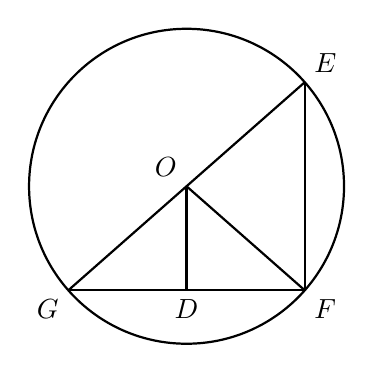
\begin{tikzpicture}[scale=1]

    % Define the center of the circle
    \coordinate (O) at (0,0);

    % Draw the main circle
    \draw[thick] (O) circle (2);

    % Define points on the circle
    % G and F are on the bottom, E is on the top right
    \coordinate (G) at (-1.5, -1.32);
    \coordinate (F) at (1.5, -1.32);
    \coordinate (E) at (1.5, 1.32);
    
    % Define point D on the segment GF, such that OD is perpendicular to GF
    \coordinate (D) at (0, -1.32);

    % Draw the line segment GF
    \draw[thick] (G) -- (F);

    % Draw the vertical line segment OD
    \draw[thick] (O) -- (D);

    % Draw the radius from O to G
    \draw[thick] (O) -- (G);

    % Draw the line segment from O to F
    \draw[thick] (O) -- (F);

    % Draw the line segment from O to E
    \draw[thick] (O) -- (E);

    % Draw the vertical line segment from E to F
    \draw[thick] (E) -- (F);

    % Add the labels for the points exactly as shown in the image
    % Using math mode ($...$) for English letters to render them properly
    \node[above left] at (O) {$O$};
    \node[below left] at (G) {$G$};
    \node[below] at (D) {$D$};
    \node[below right] at (F) {$F$};
    \node[above right] at (E) {$E$};

\end{tikzpicture}